\subsection{VNPay Sandbox và xác minh kết quả}
\label{sec:vnpay-design}
Tích hợp VNPay sử dụng ba thành phần: frontend hiển thị QR/liên kết và trạng thái; NestJS tạo yêu cầu, kiểm chứng kết quả và ghi sổ; VNPay Sandbox xử lý phiên thanh toán thử. QR chứa URL mở trang VNPay, không phải QR chuyển khoản trực tiếp của ứng dụng ngân hàng. Chữ ký và khóa merchant chỉ được xử lý ở backend. Cách phân biệt Return/IPN và quy tắc tham số được đối chiếu với tài liệu VNPay~\cite{VNPAYPAY,VNPAYFAQ}.

\subsubsection{Phân biệt đơn hàng, lần thanh toán và khoản áp dụng}
\begin{table}[htbp]\centering\small
\begin{tabularx}{\linewidth}{|p{.30\linewidth}|X|}\hline
\textbf{Thực thể} & \textbf{Trách nhiệm}\\\hline
Order & Nghĩa vụ phục vụ và tiền còn cần thu: total trừ creditApplied. Một đơn có thể thử thanh toán nhiều lần.\\\hline
VnpayAttempt & Mỗi lần giao dịch có txnRef duy nhất, số tiền, URL, hạn, mã giao dịch nhà cung cấp và trạng thái riêng; giữ lịch sử cả lần thất bại/chưa rõ.\\\hline
PaymentStartRequest & Ánh xạ cặp khách/key tới attempt để gửi lại yêu cầu không tạo thêm lần thanh toán. Key mới vẫn có thể tái dùng mã đang hiệu lực.\\\hline
Payment & Khoản đã xác minh và áp dụng vào Order; không tạo cho mọi attempt hoặc tiền thu nhưng không thể phục vụ. Liên kết attempt duy nhất chống ghi nhận lại cùng lần.\\\hline
PaymentAudit & Nhật ký tạo mã, tra cứu, nhận kết quả và thao tác hỗ trợ; phục vụ truy vết theo attempt, actor và thời gian.\\\hline
PaymentRefundCase & Hồ sơ khoản đã thu nhưng không áp dụng được (thu trùng, đơn không còn hiệu lực); một hồ sơ theo attempt, quầy xử lý bằng chứng từ.\\\hline
\end{tabularx}\caption{Phân tách dữ liệu thanh toán để bảo toàn lịch sử và tránh ghi nhận trùng}
\end{table}

Ví dụ đơn 75.000đ đã chuyển credit 45.000đ chỉ cần thu thêm 30.000đ. Backend ký đúng phần còn thu; frontend không tự quyết định số tiền. Nếu lần A hết hạn rồi cấp B và cả hai cùng thu thành công, chỉ một khoản được áp dụng cho đơn; khoản còn lại có attempt và hồ sơ xử lý riêng, không tạo hai đơn pha chế.

\subsubsection{Luồng và các nhánh kết quả}
Backend kiểm chủ đơn, PENDING/PAYMENT\_FAILED, deadline và snapshot chưa hoàn trước khi cấp mã. Lần mới có txnRef riêng; amount lưu VND nguyên, trường vnp\_Amount gửi sang cổng nhân 100 theo giao thức. Các trường được chuẩn hóa và ký HMAC-SHA512. Hạn QR bị giới hạn bởi deadline giữ món đã trình bày ở mục~\ref{sec:inventory-demand}.

Return xác minh chữ ký, merchant, tham chiếu và số tiền rồi trả HTTP 303 về trang Order; không chuyển PAID. IPN là thông báo server-to-server; QueryDr là truy vấn backend chủ động khi cần kiểm tra. Cả hai kết quả đã xác minh được quy về apply để cùng kiểm soát ghi nhận. Mất Return hoặc khách đóng tab không xóa kết quả đã commit.

\begin{table}[htbp]\centering\small
\begin{tabularx}{\linewidth}{|p{.32\linewidth}|X|}\hline
\textbf{Tình huống} & \textbf{Xử lý trong hệ thống}\\\hline
Thành công, đơn còn đủ điều kiện & Ghi Payment, PAID và điểm trên tiền mới trong cùng transaction; không giữ kho thêm.\\\hline
Thất bại đã xác minh & Ghi FAILED/EXPIRED theo kết quả; đơn còn hạn có thể bắt đầu lần khác.\\\hline
Timeout hoặc kết quả chưa rõ & Giữ lịch sử PENDING/REVIEW, không tự suy ra thất bại. QueryDr chạy ngoài transaction; việc cấp mã mới tuân điều kiện hạn mã/đơn và bằng chứng tiền đã thu.\\\hline
QR hết hạn, đơn còn hạn & Thử tra cứu rồi có thể cấp lần mới dù tra cứu chưa kết luận; giữ attempt cũ để nhận kết quả muộn.\\\hline
IPN lặp hoặc đến ngược thứ tự & Kết quả đã ghi không được ghi lại/cộng điểm lại; thông báo thất bại đến sau không hạ PAID.\\\hline
Thu trùng hoặc tiền về sau khi đơn không còn hiệu lực & Ghi REVIEW và hồ sơ khoản thu không áp dụng; không tự mở lại đơn/pha chế.\\\hline
\end{tabularx}\caption{Quy tắc xử lý kết quả VNPay và thanh toán lại}
\end{table}

\begin{figure}[htbp]\centering
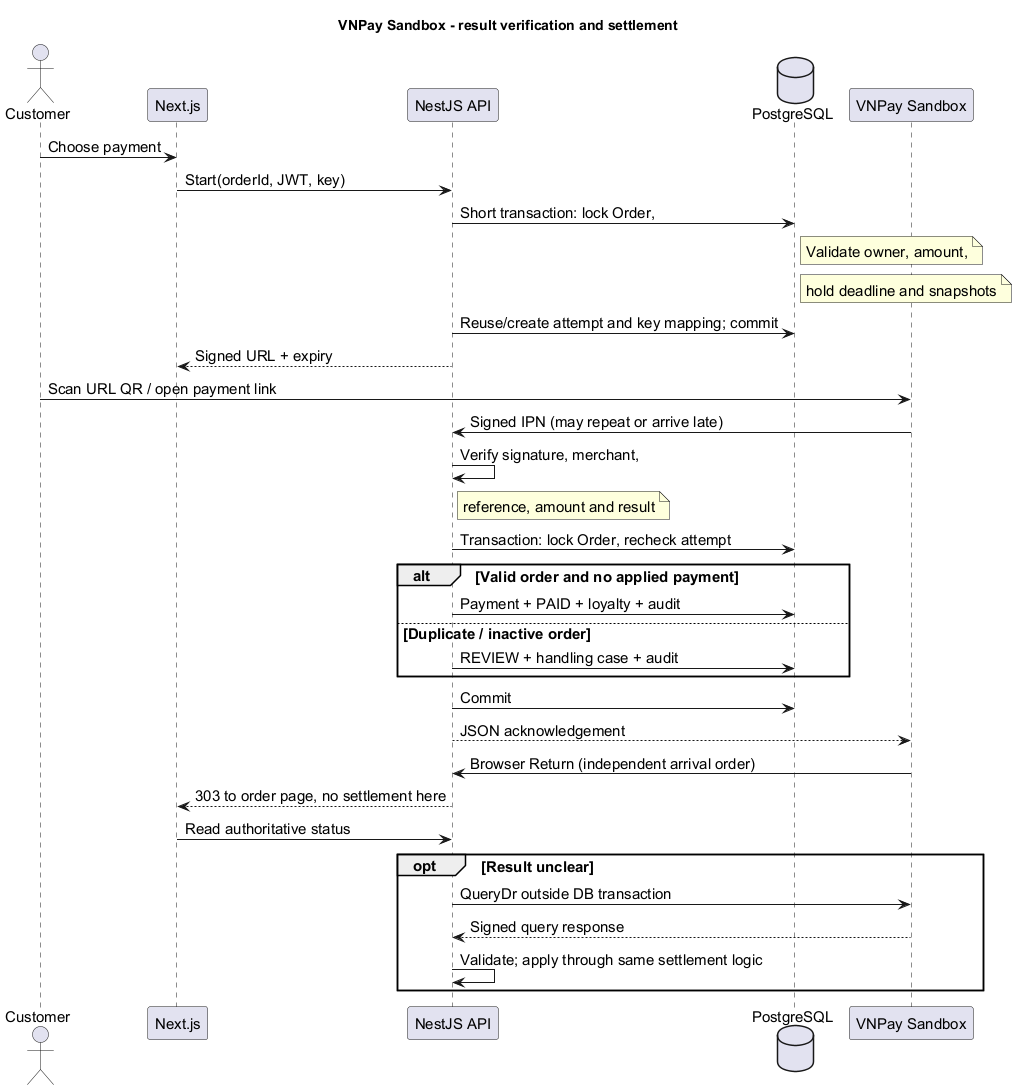
\includegraphics[width=\linewidth,height=.62\textheight,keepaspectratio]{assets/vnpay/vnpay-sequence.png}
\caption{Luồng VNPay: Return điều hướng, IPN/QueryDr xác minh và ghi nhận tại backend}
\end{figure}


\subsection{Giữ kho và hoàn theo snapshot}
\subsubsection{Định lượng theo size và topping}
\label{sec:inventory-demand}
Với mỗi dòng món, backend lấy định lượng size S từ Recipe. Chính sách định lượng đang dùng có hệ số S = 100\%, M = 125\%, L = 150\%; đây là cấu hình nghiệp vụ, độc lập phụ thu giá size. Thành phần có scalesWithSize=true được nhân hệ số rồi làm tròn lên theo từng ly. Thành phần có scalesWithSize=false giữ nguyên lượng. Sau đó cộng định lượng topping của một ly và nhân số ly; cuối cùng gộp tất cả dòng theo ingredientId.

Gọi $q_{ig}$ là lượng cơ bản nguyên liệu $g$ của món $i$, $r_s$ là hệ số size, $n_i$ là số ly và $t_{ig}$ là tổng lượng nguyên liệu $g$ từ topping của một ly. Khi thành phần tăng theo size:
\[
 D_g=\sum_i n_i\left(\left\lceil q_{ig}r_s\right\rceil+t_{ig}\right).
\]
Nếu không tăng theo size, thay $\lceil q_{ig}r_s\rceil$ bằng $q_{ig}$. Việc làm tròn trước khi nhân số ly bảo đảm mỗi ly đều có đủ lượng theo định mức nguyên.

\begin{table}[htbp]\centering\small
\begin{tabularx}{\linewidth}{|X|c|c|}\hline
\textbf{Thành phần} & \textbf{Một ly M} & \textbf{Hai ly M}\\\hline
Cà phê cơ bản 18g, tăng theo size & $\lceil18\times1{,}25\rceil=23$g & 46g\\\hline
Topping dùng thêm 5g cùng nguyên liệu & 5g & 10g\\\hline
Ly nhựa, không tăng theo size & 1 cái & 2 cái\\\hline
Tổng cà phê phải giữ & 28g & 56g\\\hline
\end{tabularx}\caption{Ví dụ minh họa cộng gộp định lượng, không phải công thức mặc định của topping Kem}
\end{table}

Hàm ingredientDemand dùng chung cho kiểm kho khi đặt và tính availability trên menu. Với lựa chọn một ly, số ly có thể bán bằng giá trị nhỏ nhất của $\lfloor stock_g/D_g\rfloor$ trên các nguyên liệu cần dùng. Do topping có thể dùng chung nguyên liệu với món, phải gộp demand trước khi chia; tính riêng hai phần rồi lấy min có thể báo còn hàng sai. Availability ở giao diện là ảnh chụp tham khảo; backend luôn kiểm lại tại transaction tạo đơn hoặc duyệt đổi món.

\subsubsection{Snapshot: vì sao không hoàn bằng công thức hiện tại?}
Recipe mô tả định mức bán hiện hành, trong khi snapshot là bằng chứng lượng đã giữ của một đơn cụ thể. Ví dụ khi đặt, một ly giữ 20g cà phê. Sau đó quầy sửa Recipe thành 25g. Nếu hủy bằng công thức mới, hệ thống cộng 25g dù trước đó chỉ trừ 20g, tạo ra 5g không có thật. Snapshot giữ quantity=20 nên hoàn đúng 20g. Thay topping, hệ số size hay chuyển công thức sang nguyên liệu khác cũng không thay đổi snapshot đã lưu.

Snapshot được tạo từ chính Map demand đã dùng để trừ kho, trong cùng transaction với Order. Không đọc lại Recipe sau bước trừ để dựng snapshot, vì lần đọc khác có thể không đại diện lượng vừa giữ. releasedAt là dấu hoàn; quantity vẫn giữ nguyên để tra cứu lịch sử. Một đơn có nhiều dòng món cùng dùng cà phê sẽ có một snapshot cà phê tổng, vì khi hủy toàn đơn chỉ cần trả đúng tổng lượng đã giữ.

\subsubsection{Hủy chủ động và hết thời gian giữ món}
Hủy chủ động kiểm tra chủ đơn, trạng thái và điều kiện thanh toán. Khách chỉ tự hủy PENDING/PAYMENT\_FAILED không có credit; backend khóa Order, kiểm tra các attempt cần xác minh, cập nhật trạng thái có điều kiện rồi release snapshot trong cùng transaction. Nếu bước hoàn bị lỗi thì trạng thái hủy cũng rollback. PAID và các trạng thái pha chế không dùng API hủy thông thường; đổi món đã trả tiền đi qua yêu cầu và quyết định của barista.

Với đơn bỏ thanh toán, reservationExpiresAt mặc định cách lúc tạo 30 phút. ReservationExpiryService quét khi khởi động và mỗi 30 giây, tối đa 100 đơn/lượt. Chỉ đóng đơn chưa trả tiền, chưa có bằng chứng đã thu và chưa sử dụng credit. Khi đủ điều kiện, worker hoàn snapshot và ghi CANCELLED cùng reservationExpiredAt; thông báo được phát sau commit. Giao diện hiển thị ``Đã hết thời gian đặt món, vui lòng đặt lại.'' và đưa khách về menu để tạo yêu cầu mua mới.

Deadline của đơn và deadline QR là hai giá trị khác nhau. Ví dụ đơn giữ món từ 10:00 đến 10:30; QR đầu hết 10:10 thì vẫn cấp QR mới trong thời gian còn giữ. Nếu tạo QR lúc 10:25, QR không được kéo dài quá 10:30. Backend kiểm deadline tại start payment và lúc áp dụng IPN, nên timer trình duyệt không quyết định quyền giữ kho.

Nếu tiền về muộn sau deadline, hệ thống giữ bằng chứng giao dịch, ghi REVIEW và mở hồ sơ xử lý khoản thu không áp dụng; không tự mở lại đơn, trừ kho lại hoặc gửi pha chế. Nếu worker chưa đóng đơn, callback xử lý việc đóng/hoàn trong transaction thích hợp. Các đơn đã chuyển credit hoặc có bằng chứng thu tiền được bảo toàn để quầy xử lý, tránh tự xóa giá trị khách đã trả.

\begin{figure}[p]\centering
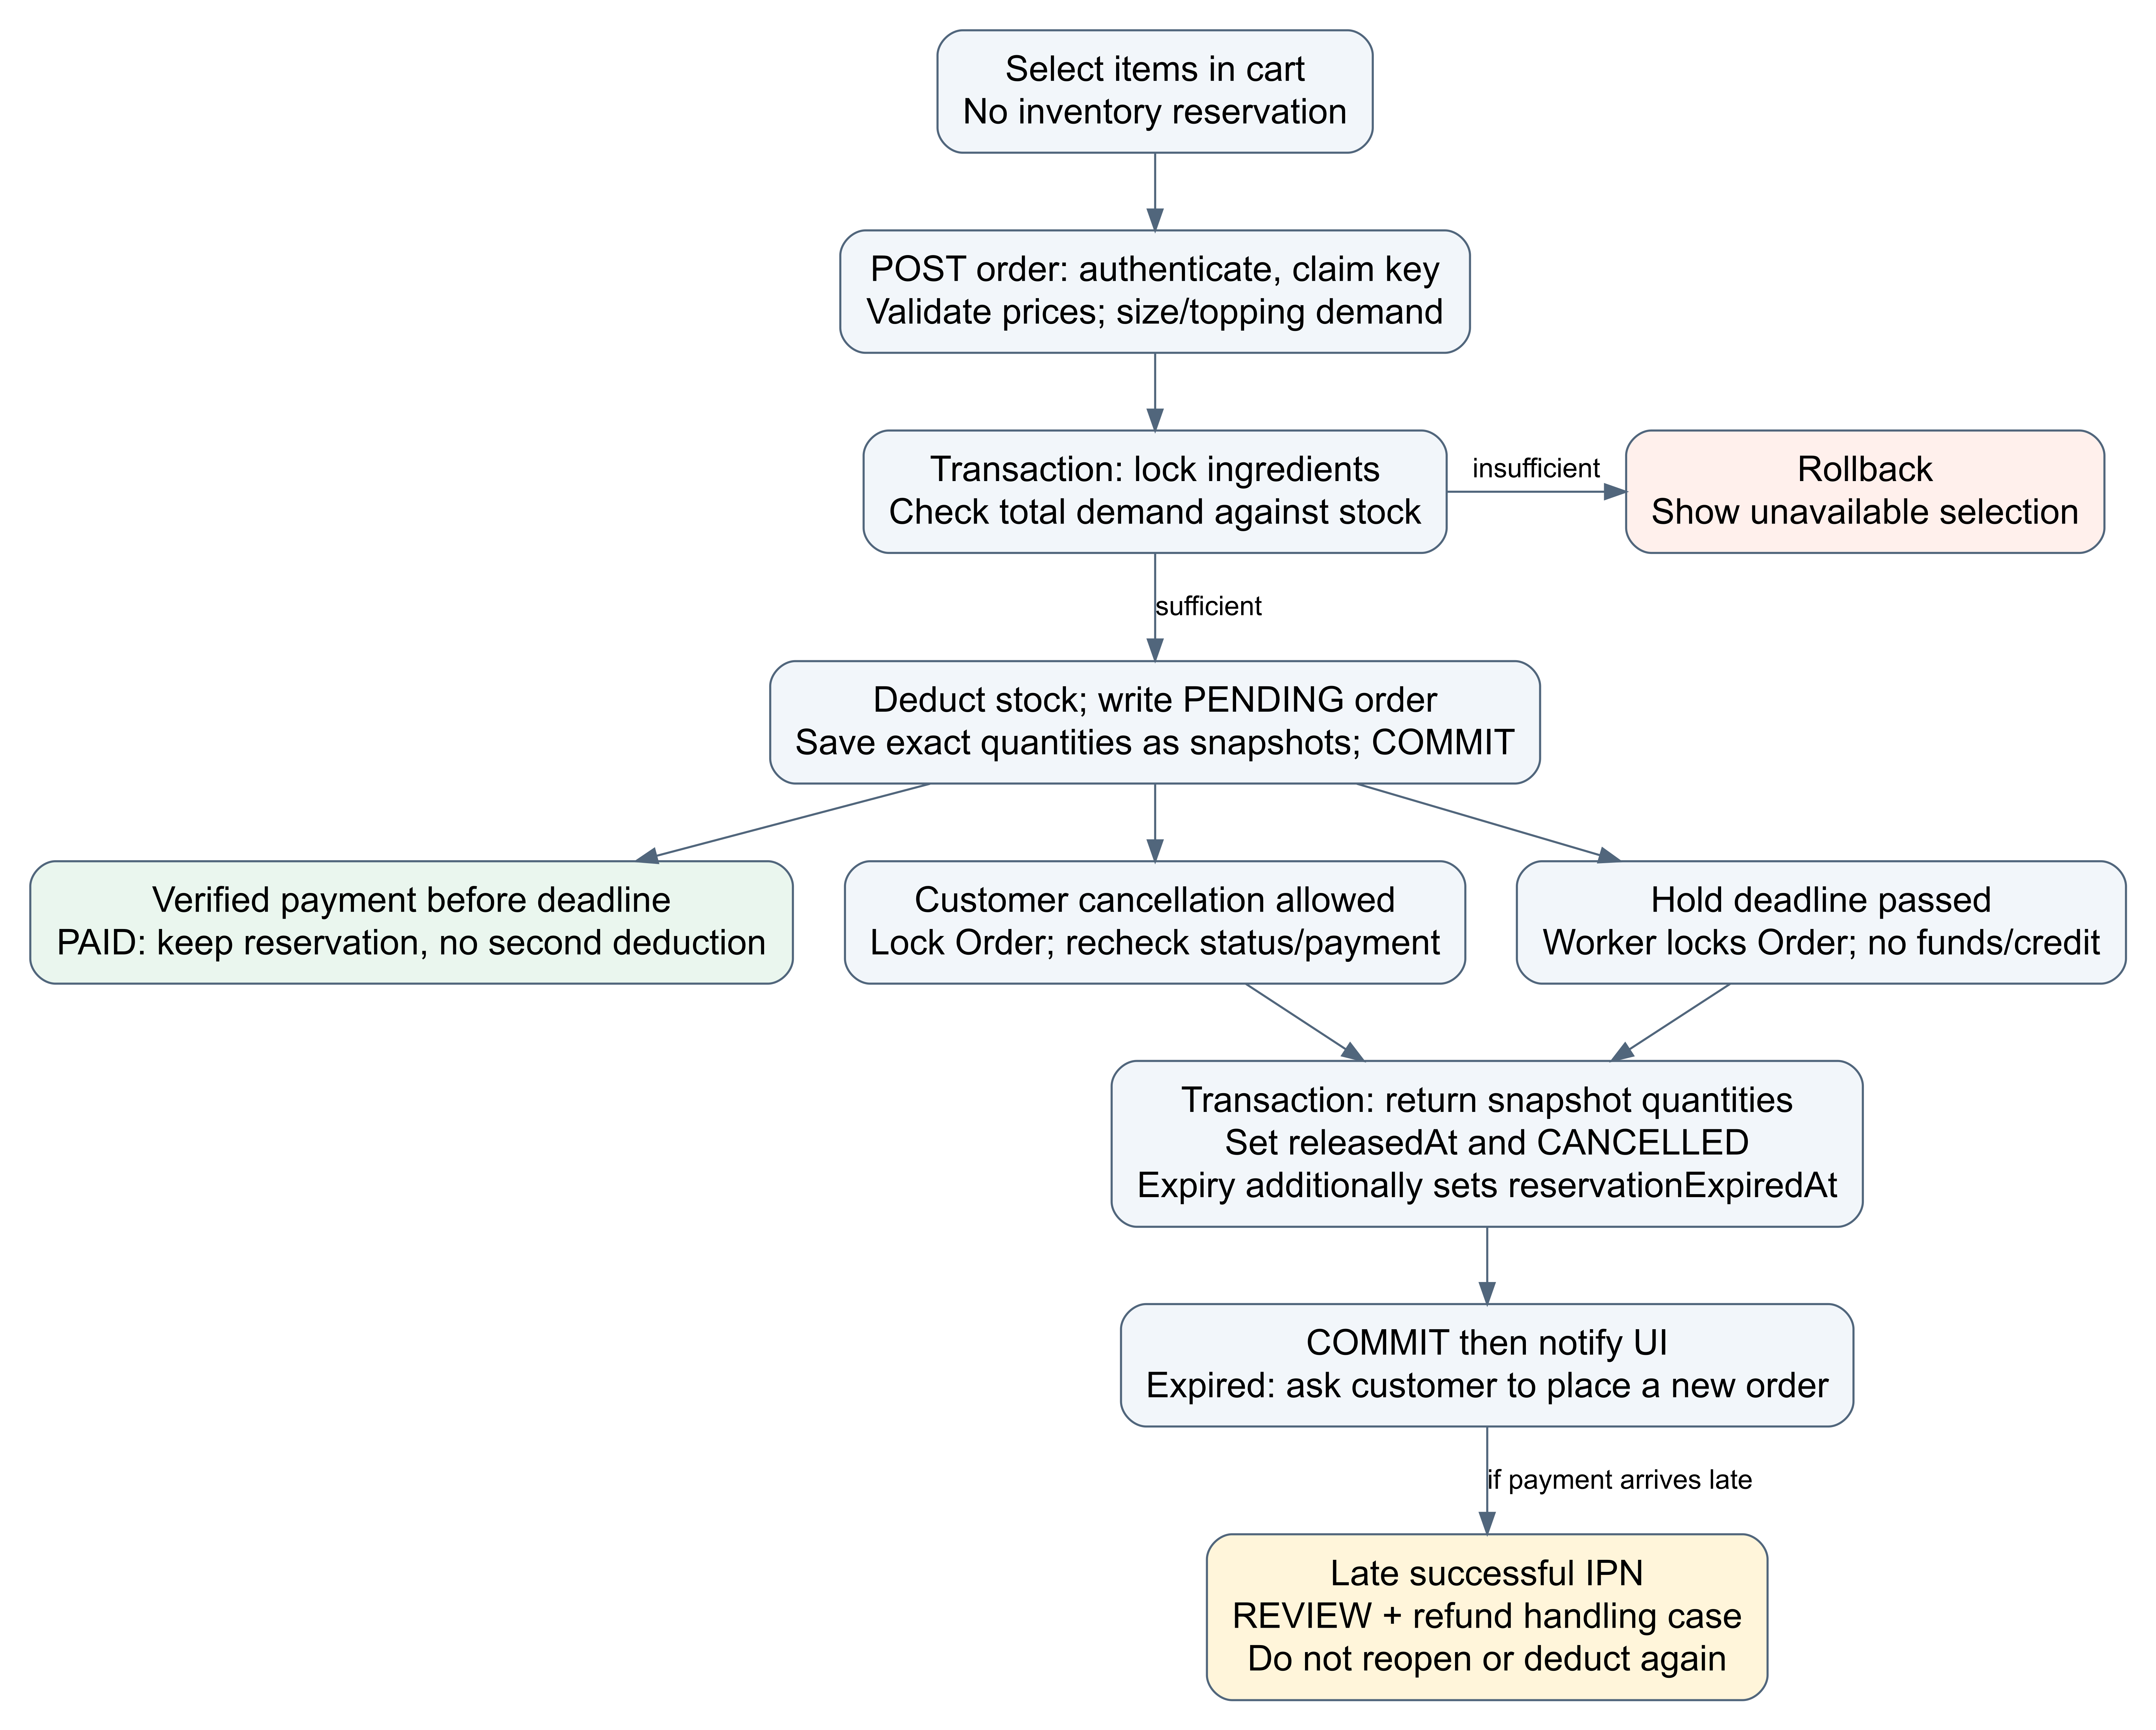
\includegraphics[width=\linewidth,height=.82\textheight,keepaspectratio]{assets/inventory/inventory-lifecycle.png}
\caption{Luồng tạo đơn, giữ kho, thanh toán, hủy và hết thời hạn giữ món}
\label{fig:inventory-lifecycle}
\end{figure}


\subsection{Đổi món, chuyển tiền và thanh toán chênh lệch}
\label{sec:exchange-design}
Đổi món là quy trình thay thế một đơn đã thanh toán trước khi pha chế, không phải khách tự hủy để nhận tiền. Khách mở liên kết hỗ trợ trên Order PAID, chọn lại món/size/topping qua menu và giỏ đổi riêng; backend báo giá, khách gửi lý do và quầy quyết định. Mở menu hoặc nhận báo giá không tự hoàn kho hay đóng đơn cũ.

\subsubsection{Dữ liệu yêu cầu và báo giá}
OrderExchange lưu sourceOrderId, replacementOrderId, items, reason, trạng thái, quyết định và version. Liên kết hai Order giữ được lịch sử trước/sau thay vì sửa trực tiếp các dòng món của đơn đã thu tiền. Unique(sourceOrderId, key) cùng requestHash bảo vệ gửi lặp yêu cầu.

quotedLines/quotedTotal lưu báo giá đã nhận khi yêu cầu được tạo. Frontend gửi expectedQuote để backend đối chiếu fingerprint của báo giá; nếu giá/trạng thái đổi trước lúc gửi, khách phải xem lại. Fingerprint là dấu vân tay đối chiếu dữ liệu, không phải chữ ký cổng thanh toán. Khi đã tạo yêu cầu, bước duyệt dùng thành tiền snapshot, tránh tính lại theo giá menu mới trong lúc khách chờ.

\begin{table}[htbp]\centering\small
\begin{tabularx}{\linewidth}{|p{.24\linewidth}|X|}\hline
\textbf{Trạng thái} & \textbf{Ý nghĩa và tác động}\\\hline
REQUESTED & Chờ quầy; đơn nguồn vẫn PAID và giữ nguyên liệu. Chặn chuyển PREPARING cho tới khi xử lý yêu cầu.\\\hline
APPROVED & Đã tạo đơn thay thế, chuyển credit và đóng đơn nguồn trong cùng transaction.\\\hline
REJECTED & Quầy từ chối, lưu ghi chú; giữ nguyên món và tiền của đơn nguồn.\\\hline
WITHDRAWN & Khách rút yêu cầu còn chờ bằng version; tiếp tục đơn nguồn.\\\hline
\end{tabularx}\caption{Vòng đời yêu cầu đổi món, độc lập vòng đời Order}
\end{table}

\subsubsection{Chuyển giá trị đã trả và thu chênh lệch}
Giá trị có thể chuyển bằng tổng Payment đã áp dụng của đơn nguồn cộng creditApplied đã chuyển vào đơn đó; backend kiểm bằng total của đơn nguồn trước khi duyệt. Credit là giá trị gắn với đơn thay thế, không phải số dư ví dùng tùy ý.

\begin{table}[htbp]\centering\small
\begin{tabularx}{\linewidth}{|X|c|c|c|}\hline
\textbf{Trường hợp} & \textbf{Tiền cũ} & \textbf{Món mới} & \textbf{Thu thêm}\\\hline
Đổi bằng giá & 45.000đ & 45.000đ & 0đ\\\hline
Đổi cao hơn & 45.000đ & 75.000đ & 30.000đ\\\hline
Đổi thấp hơn & 45.000đ & 40.000đ & Yêu cầu chọn lại\\\hline
\end{tabularx}\caption{Ví dụ credit và số tiền thu thêm khi đổi món}
\end{table}

Order mới giữ total bằng giá trị món, creditApplied bằng tiền chuyển, amountDue bằng phần chênh lệch. Đổi bằng giá tạo Order PAID nhưng không tạo Payment giả hoặc cộng điểm trên tiền cũ lần nữa. Đổi cao hơn tạo Order PENDING; VNPay chỉ thu phần chênh lệch và điểm tính trên tiền mới. Quy tắc hiện tại không áp voucher mới trong yêu cầu đổi; phần thu dương qua tích hợp VNPay phải từ 5.000đ. Quầy chỉ bắt đầu pha khi đơn thay thế đã đủ tiền.

\begin{figure}[htbp]\centering
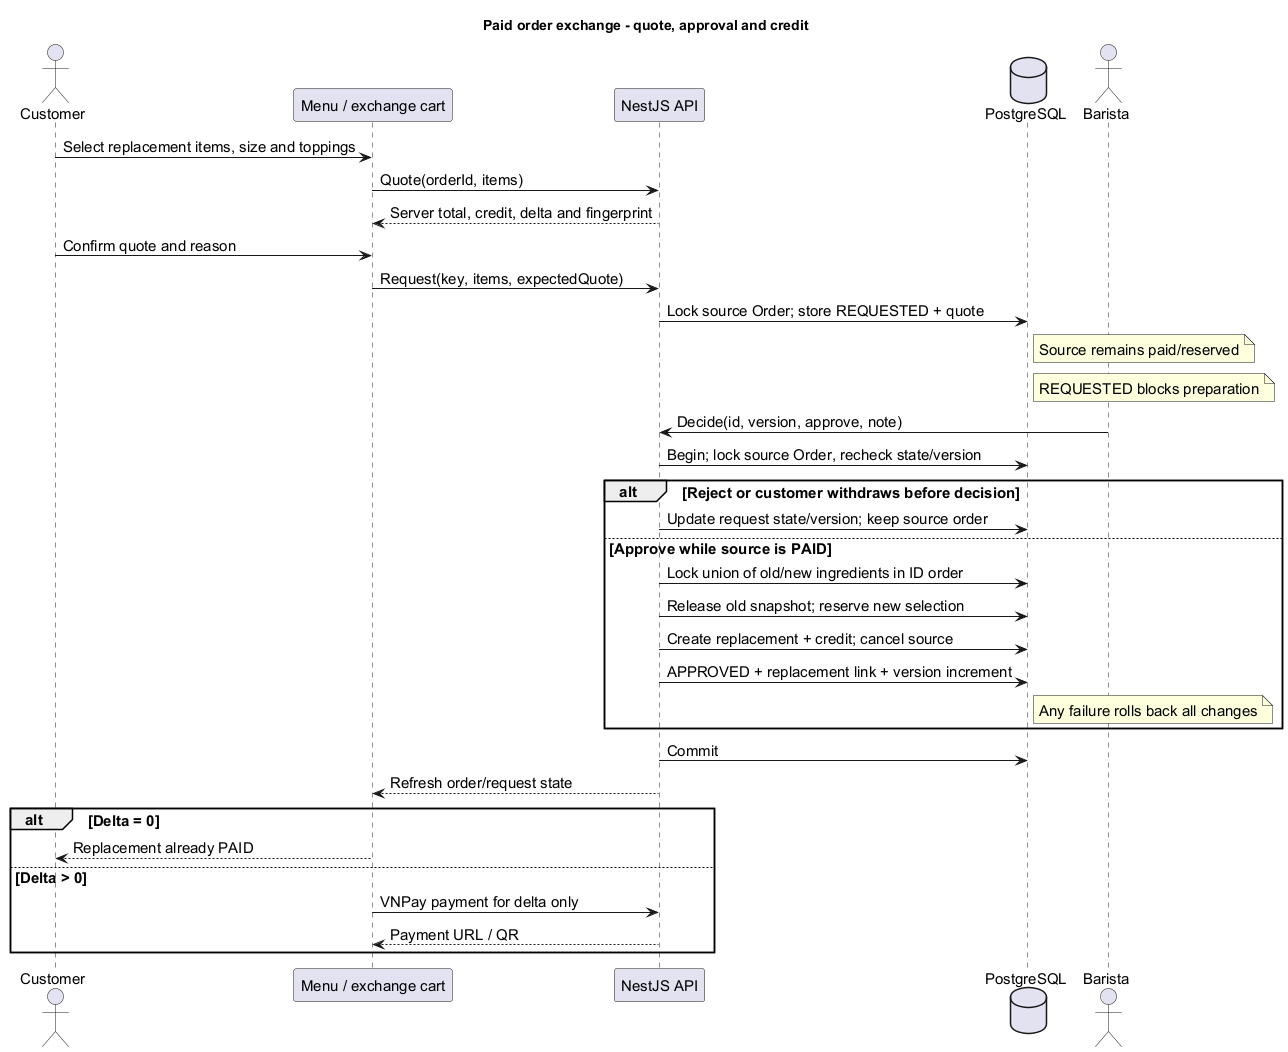
\includegraphics[width=\linewidth,height=.56\textheight,keepaspectratio]{assets/exchange/exchange-sequence.png}
\caption{Khách gửi yêu cầu, quầy quyết định, transaction thay đơn và thanh toán chênh lệch}
\end{figure}


\subsection{Version trong hồ sơ xử lý và khoản thu dư}
OrderExchange và PaymentRefundCase dùng version để phát hiện cập nhật trên dữ liệu cũ. Hai nhân viên cùng đọc version=0: người ghi trước cập nhật với điều kiện id/version/trạng thái rồi tăng lên 1; người còn lại bị 409. Đây là optimistic concurrency cho hồ sơ; việc giữ nguyên liệu sử dụng khóa dòng trong transaction.

PaymentRefundCase liên kết duy nhất với attempt đã thu nhưng không áp dụng được. Quy trình OPEN, PROCESSING, COMPLETED có ghi chú, người xử lý, thời gian và chứng từ duy nhất. Nhân viên thực hiện chuyển trả bên ngoài rồi ghi nhận bằng chứng; backend theo dõi bằng chứng từ và nhật ký xử lý. Thu trùng khác với khách đổi ý sau trả tiền và không bị ép sử dụng khoản dư để mua món khác.
